\documentclass{foi}
\usepackage[utf8]{inputenc}
\usepackage{lipsum}
\usepackage{float}


\vrstaRada{\projekt} % \diplomski \projekt \seminar \zavrsni
\title{Simulacija sustava najma električnih vozila}

\author{Leo Leljak}
\spolStudenta{\odaberi} % \zensko ili \musko
\mentor{Bogdan Okreša Đurić}
\spolMentora{\odaberi} % \zensko ili \musko
\godina{2022}
\mjesec{travanj}
\date{2021}
%\status{izvanredni}
\indeks{0016122912}
\smjer{Informacijsko i programsko inženjerstvo} % (ili Poslovni sustavi, Ekonomika poduzetništva, Primjena informacijske tehnologije u poslovanju, Informacijsko i programsko inženjerstvo, Baze podataka i baze znanja, Organizacija poslovnih sustava, Informatika u obrazovanju)
\titulaProfesora{Dr. sc.}

\sazetak{U ovome radu biti će implementiran sustav najma električnih vozila. Sustav će se sastojati od tri agenta. Prvi agent je centralni sustav koji upravlja prijavom neke stanice u sustav najma vozila, te se takav agent može više puta pokrenuti ukoliko nam je potrebno više različitih stanica. Drugi agent je sama stanica koja će se sastojati od dva različita ponašanja, te upravlja zahtjevima pojedinih klijenata koji žele iznajmiti vozilo. U radu ćemo proći detaljnjije kroz samu strukturu pojedinih agenata kao i način njihove implementacije. Posljednji agent je krajnji korisnik koji unajmljuje vozila, te ih koristi. Agent krajnjeg korisnika biti će kreiran kao konačni automat te ćemo također kroz njegovu implementaciju proći detaljnjije u radu.
\\ \\ U samom radu proći ćemo kroz arhitekturu rješenja kao i detalje implementacije pojedinog agenta i njegovih ponašanja. Rezultat je skalabilno rješnje koje se može lako proširiti dodatnim agentima pošto se stvara decentralizirani sustav najma vozila.}

\kljucneRijeci{agent, simulacija, električna vozila, komunikacija, python}

\begin{document}

\maketitle

\tableofcontents

\pagestyle{plain}
\chapter{Uvod}

Simulacija sustava iznajmljivanja električnih vozila može biti izvedena na više različitih načina. U ovome radu koristimo pojednostavljeni pristup u kojemu se ne dotičemo procesa planiranja i zakazivanja pojedinih narudžba u određeno vrijeme pošto to nije u opsegu ovoga rada. Glavni je fokus na kreiranju različitih ponašanja koji su potrebni kod agenata koje implementiramo. Također koriste se različite vrste ponašanja - ciklično, periodično te konačni automat. U ovome radu prikazana je unakrsna komunikacija između klijenata kao i decentralizirani pristup kreiranja novih agenata u sustav iznajmljivanja električnih vozila. Na taj način sustav je skalabilniji te se može lakše nadodati novi agent, a da svi ostali agenti (pojedinačne postaje) znaju za novog agenta. Postoji jedan centralni agent koji zaprima nove stanice koje se žele uključiti u posao iznajmljivanja, no nakon toga svaka je stanica neovisna o centralnom sustavu što se tiče poslovanja i iznajmljivanja. 

Električna vozila zbog svoje zelene tehnologije koju koriste sve su poželjnija vrsta prijevoznog sredstva kojeg krajnji korisnik želi unajmiti. Unutar rada koristi se 4 vrste električnih automobila i 3 vrste električnih bicikala, svaki sa svojim svojstvima kao što su maksimalni domet, dnevna cijena najma, trenutna napunjenost baterije i ostalo. Kasnije će se detaljnjije proći kroz sam opis svojstva i njihovu važnost unutar cijelokupnog sustava najma električnih vozila. Lista vozila proširiva je no za potrebu ovog rada smanjena je na 8 vozila ukupno kako bi fokus bio na arhitekturi rješenja kao i samoj komunikaciji između agenata.

\chapter{Metode i tehnike rada}

Agenti su implementirani u programskom jeziku Python korištenjem biblioteke “Smart Python Agent Development Environment" (SPADE) . SPADE je idealna biblioteka za implementiranje ovoga rješenja, a može se koristiti sa Pythonom 3.6, te biblioteka koristi asyncio i striktno slijedi principe PEP8 i Clean Code. [1]

Tijekom vježbi na kolegiju Višeagentni sustavi korištene su iste tehnologije, te slične tehnike rada. Na vježbama smo se mogli upoznati sa raznim ponašanjima koji se mogu koristiti i implementirati. Gotovo svako od tih ponašanja iskorišteno je u ovome radu pošto je simulacija iznajmljivanja električnih vozila idealan kandidat da bi se unutar strukture rješenja implementirale razne vrste ponašanja agenta. Tako je su u ovom radu korištena ponašanja kao što su ciklično, periodično i ponašanje konačnog automata. 

Korištene su paradigme objektnog programiranja. Kod je iskoristiv te za pokretanje više različitih klijenata koristi se parsiranje ulaznih argumenata kako bi se id i lozinka agenta mogla definirati prilikom pokretanja agenata. Na taj način moguće je pokrenuti više različitih agenata svaki sa svojim korisničkim podacima. Neki dijelovi koda su dokumentirani kako bi se čitaoc mogao lakše snalaziti prilikom pregleda izvornog koda sustava iznajmljivanja električnih vozila.

\chapter{Opis sustava i pregled stanja agenata}

U ovom dijelu opisan je način rada sustava za najam električnih vozila kao i interakcija između agenata. Proći će se kroz teorijsku podlogu višeagentnih sustava te će se nakon toga prijeći na shematski prikaz ponašanja koje agenti imaju. Sustav se sastoji od centralnog agenta, agenta stanica te pojedinačnih klijenata koji mogu izvršiti narudžbu. Klijent je napravljen preko ponašanja konačnog automata pa će i određene naglasak biti na izvedbi toga dijela.

\section{Višeagentni sustavi}

Prema [2] paradigma višegentnih agenata vezana je uz autonomne, reaktivne entitete koje mogu djelovati individualno i izvršavati specifične zadaće koje su mu dane. Agenti su odlični izvršioci zadaća za koje su namijenjeni te mogu samostalno određivati načine na koji dolaze do ciljeva. Ti načini mogu biti implementirani kao složen algoritam koji agent slijedi ili može postojati određena baza znanja na temelju koje agent odlučuje kako stići do cilja.

\begin{figure}[h!]
    \centering
    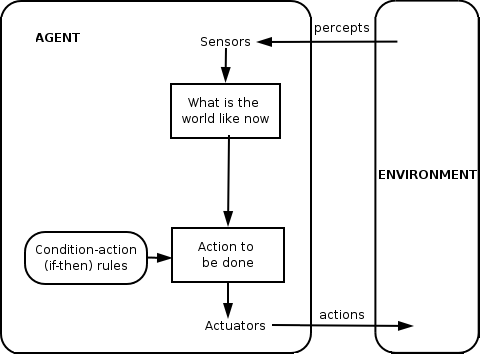
\includegraphics[width=0.7\textwidth]{slike/agentReakcije.png}
    \caption{Dijagram jednostavnog reaktivnog agenta (Izvor: Wikipedia, 2022)}
    \label{fig:dijagramAgenti}
\end{figure}

Na slici 1 može se vidjeti shematski primjer jednog agenta koji ima interakciju za svojom okolinom. Agent reagira na promjene okoline preko senzora te postoji zadan set if-then pravila prema kojima on reagira i vrši određene zadaće. Ovdje se radi o primjeru jednostavnog reaktivnog agenta. 

\begin{figure}[h!]
	\centering
	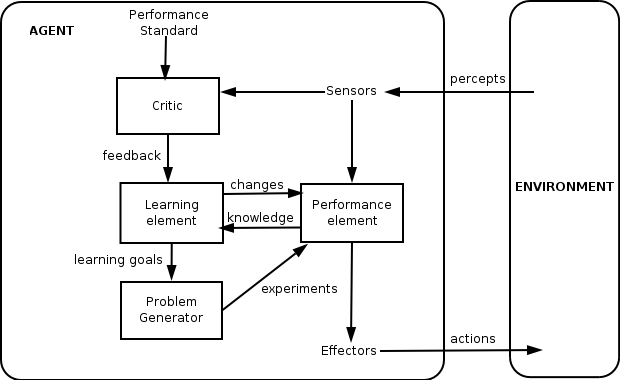
\includegraphics[width=0.7\textwidth]{slike/agentUcenja.png}
	\caption{Dijagram jednostavnog agenta učenja (Izvor: Wikipedia, 2022)}
	\label{fig:dijagramAgenti}
\end{figure}

Na slici 2 vidimo shematski prikaz agenta učenja (eng. Learning agent). Radi se o agentu koji nije samo izvršioc zadataka prema nekom jasnom setu if-then pravila već ima određene ciljeve učenja te pri svakoj interakciji se stvara novi zapis u bazu znanja kako bi već pri sljedećoj interakciji mogao bolje odreagirati na promjene.

Agenti imaju nekoliko mogućih fleksibilnosti - reaktivni, proaktivni te društveni. Reaktivni ageenti su oni koji ostvaruju kontinuiranu interakciju sa svojom okolinom te pravovremeno reagiraju na promjene koje se događaju unutar takve okoline. Proaktivni agenti su agenti koji su pogonjeni ciljevni, tj. Nisu pogonjeni isključivo događajima u okolini. Posljedna moguća fleksibilnost agenta je društevnost koja je sposobno interakcije agenta s drugim agentima putem nekog jezika za komunikaciju.

Često se stavljaju višeagentni sustavi u kontekst umjetne inteligencije te isto tako i ekspertnih sustava. Kod višeagentnih sustava u odnosu na ekspertne sustave razlika je u tome da ekspertni sustavi sadrže informacije, dok agenti nisu stvoreni za pohranjivanje informacija nego izvršavanje nekih konkretnih zadataka. Umjetno inteligencija najčešće ima intenciju oponašati razne situacije koje se nalaze u stvarnom svije, dok su agenti tu da izvršavaju neke jednostavije operacije za koje su namijenjeni.

\section{Komunikacija između agenata}

Općenito je komunikacija između agenata ključna kod razvoja bilo kojeg višeagentnog sustava. Za ovaj projekt koristi se komunikacija prema FIPA ACL standardu koji se također koristio tijekom vježbi na kolegiju Višeagentni sustavi. Na taj način svi agenti međusobno mogu komunicira preko jasnih poruka, te je komunikacija jednostavna. U ovom projektu svi agenti moći će zaprimiti poruku kao i poslati istu prema drugom agentu.
\pagebreak

\section{Sustav najma električnih vozila}

U ovome poglavlju prikazan je predloženi sustav najma električnih vozila. Sustav je pojednostavljen kako bi u fokusu bila komunikacija između agenata, njihova interakcija te pojedina ponašanja agenata. Sustav se sastoji od tri glavna agenta:

\begin{itemize}
	\item Rent Central
	\item Rent Station
	\item User
\end{itemize}

\begin{figure}[h!]
	\centering
	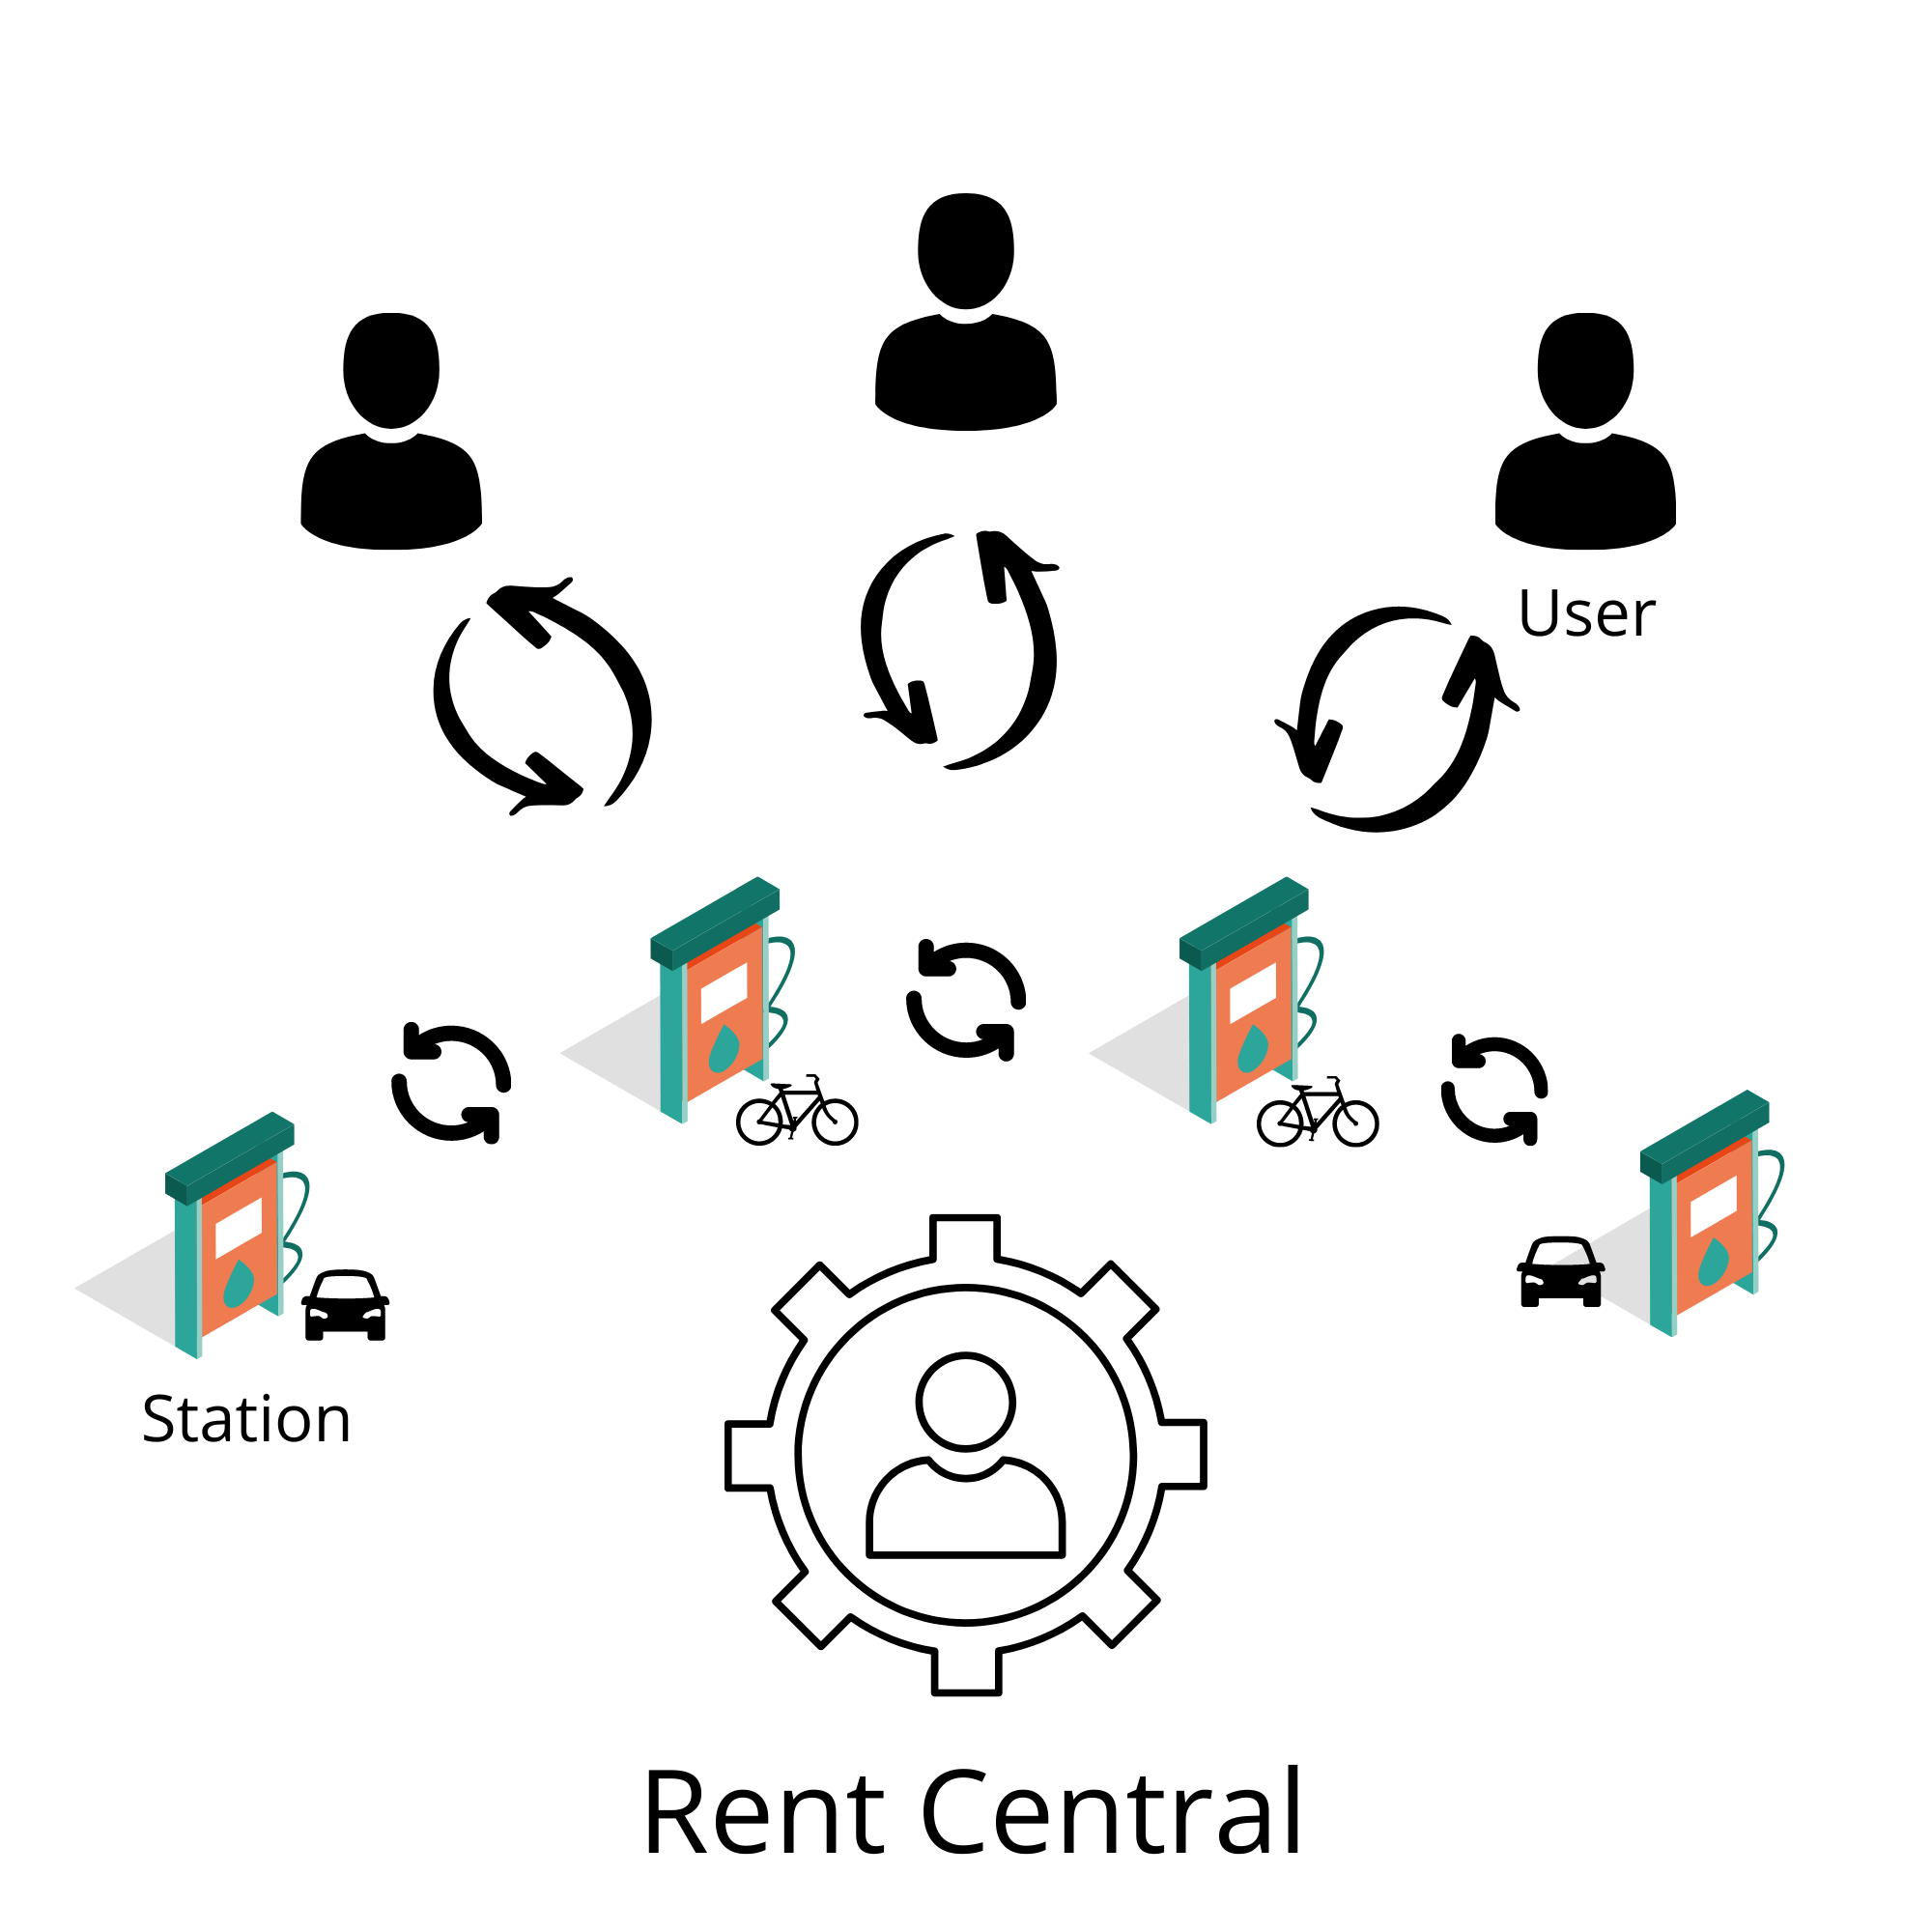
\includegraphics[width=0.7\textwidth]{slike/rentCentral.png}
	\caption{Dijagram sustava agenata (Izvor: U vlastitoj izvedbi, 2022)}
	\label{fig:dijagramAgenti}
\end{figure}

Unutar sustava postoje tri ključna agenta. Prvi agent Rent Central potrebno je pokrenuti samo jedamput i njegova je namjena da bude glavna tvrtka u koju se mogu učlaniti ostali Rent Stationi. Glavna centrala zadužena je za zaprimanje zahtjeva od Rent Stationa kod početne prijave samih stanica. Kada se prijavi nova stanica u sustav stanica svoj se stanici distribuira poruka o skupu svih trenutno prijavljenih i aktivnih stanica u sustav. 

Na taj način se pokušava decentralizirati sustav. Alternativno tome pristupu bio bi potpuno centralizirani sustav a više o tome u sljedećem potpoglavlju. Krajnji korisnik kada želi unajmiti određeno električno vozilo (bicikl, automobil) može to učini direktno zahtjevom prema željenoj stanici. Ukoliko željena stanica nema vozilo koje korisnik želi unajmiti, ili je vozilo trenutno na punjenju tada stanica uzima neku drugu stanicu iz liste svih trenutno dostupnih stanica i pruža tu informaciju korisniku. U tom slučaju korisnik je obavješten porukom na koju je stanicu upućen.

\section{Decentralizirani pristup}

Postoje više različitih pristupa izradi ovakvog sustava. U ovome radu korištena je varijanta decentraliziranog pristupa gdje svaka stanica zna za svaku stanicu i može međusobno komunicirati sa njom. Glavna centrala (Rent Central) zadužena je za mogućnost prijave posebnih stanica (Rent Station-a) u sustav najma električnih vozila. Taj dio je ostao centraliziran zbog razloga što mora postojati centralni sustav koji nadzire rad ostalih stanica. Također ukoliko bi to bio sustav koji radi na principu franšize, svaka stanica se mora pojedinačno prijaviti u takav sustav. Kada se pojedinaca stanica prijavi kod Rent Centrala, centralna stanica javlja svim ostalim stanicama koje su trenutno prijavljene trenutni skup svih prijavljenih stanica. Svaka stanica zaprimi trenutni skup svih prijavljenih stanica te ažurira svoje podatke o njima. Na taj način svaka stanica zna za sve stanice koje su trenutno prijavljene u njenoj okolini.

\begin{figure}[h!]
	\centering
	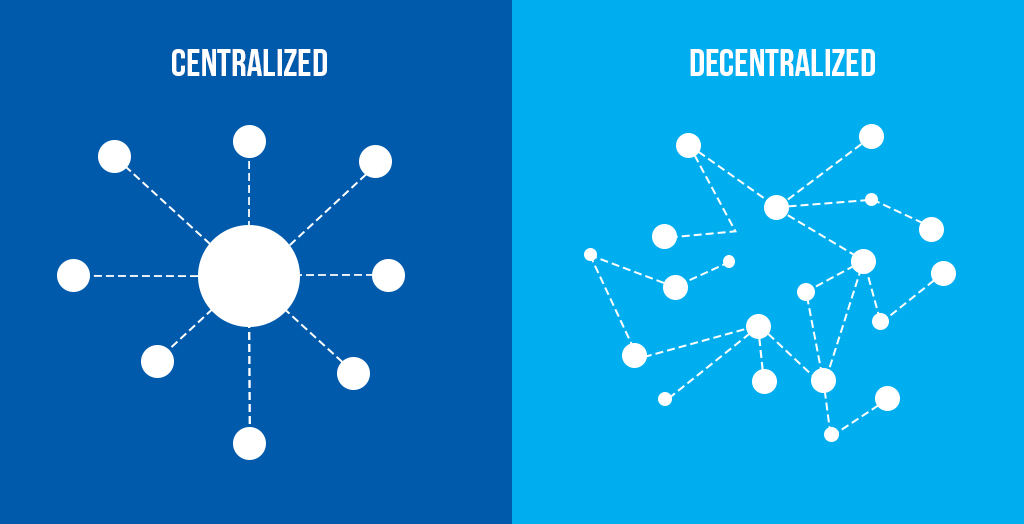
\includegraphics[width=0.7\textwidth]{slike/decentralized.jpg}
	\caption{Dijagram sustava agenata (Izvor: aceinfoway.com/blog/centralized-vs-decentralized-apps, 2022)}
\end{figure}

Alternativan pristup odabranome bio bi potpuno centralizirani sustav gdje bi Rent Central jedini znao za sve stanice koje su trenutno prijavljenje u sustav. Na taj način bi svaki zahtjev nekoj drugoj stanici preko izvorne stanice morao ići preko centralnog sustava. Na taj način bi se stvorilo veće opterećenje na centralni sustav pošto bi svi zahtjevi išli preko njega. Decentraliziranim pristupom također eliminiramo jednu točku kvara (eng. Single point of failure). Stanice nisu ovisne o jednoj centralnoj stanici te u slučaju da dođe do kvara na centralnoj stanici, svaka stanica može nezavisno djelovati.
\pagebreak

\section{Rent Central Agent}

Centralni agent jedini je dio koji je na neki način centraliziran zbog svoje zadaće koje izvršava. Na ovog agenta može se gledati kao na tvrtku koja prodaju svoja prava na rentanje električnih vozila drugim stanicama. 

Agent ima samo jedno ponašanje koje je ciklično. Ciklično ponašanje je poput petlje koja se ponavlja. Postoje tri glavne zadaće, odnosno zahtjeva koje ovo ponašanje može primiti:
\begin{itemize}
	\item Register station
	\item Unregister station
	\item Update earnings
\end{itemize}

\begin{figure}[h!]
	\centering
	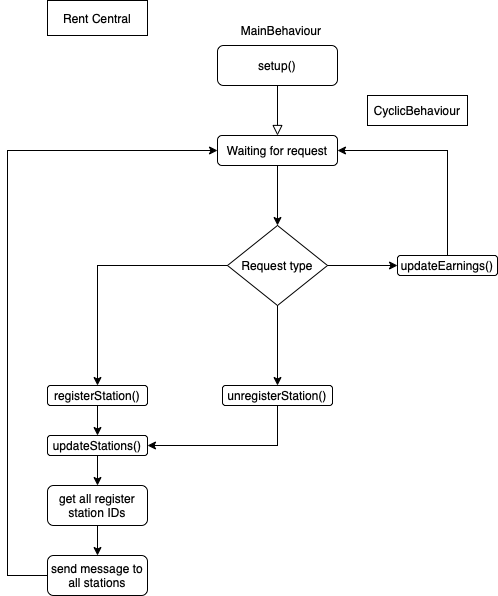
\includegraphics[width=0.7\textwidth]{slike/rentCentralSheme.png}
	\caption{Dijagram agenta RentCentral (Izvor: U vlastitoj izvedbi, 2022)}
\end{figure}

\textbf{Register station} zahtjev šalju stanice kada se žele registrirati u sustav i dobiti informacije o svim drugim stanicama koje se trenutno nalaze u sustavu iznajmljivanja električnih vozila. Kada je takav zahtjev zaprimljen tada se u listu sprema id novoregistrirane stanice te se šalje poruka svim trenutno registriranim stanicama sa trenutnom listom registriranih stanica. Na taj način svaka stanica je obavještena o trenutno registriranim stanicama te svaka stanica zna za svaku stanicu i može izravno komunicirati sa njom preko jedinstvenog id-a stanice.

\textbf{Unregister station} radi suprotnu stvar od sestrinske register station opcije. Naime sa ovim zahtjevom stanica šalje zahtjev za deregistracijom te se iz liste briše takva stanica i ponovno se šalje svim stanicama ažurirana lista svih aktivnih stanica.

\textbf{Update earnings} zahtjev šalju stanice u određenim intervalima. To je definirano ponašanje unutar agenta Rent Stationa kroz koje će se proći u detaljima vezanim uz strukturu agenta Rent Station.

\section{Rent Station Agent}

Rent Station agent sastoji se od dva ponašanja koja su različita po svojim svojstvima. Prvo ponašanje je ciklično ponašanje koje se ponavlja u petlju, te mu je glavna uloga čekanje zahtjeva i regiranje na iste. Drugo ponašanje koje ovaj agent ima je periodično ponašanje, a njegova ključna uloga je izvršavanje periodičnog punjenja baterija električnih vozila. U određenim intervalima takvo ponašanje provjerava trenutno stanje vraćenih vozila te za ona vozila kojima je potrebno punjenje takvo punjenje izvršava.

\textbf{Glavno ciklično ponašanje} sastoji se od ukupno 4 zahtjeva koje može obraditi:
\begin{itemize}
	\item Update station data
	\item Reserve vehicle
	\item Collect vehicle
	\item Return vehicle
\end{itemize}

Na slici NAPIŠI BROJ SLIKE može se vidjeti dijagram prvog ponašanja koje ovaj agent ima. Takvo ponašanje je ciklično, a na samom početku vrše se određene pred radnje. Prisjetimo se da se ovdje radi o stanici za najama električnih vozila koja se na samom početku nakon pokretanja mora registrirati u sustav najama električnih vozila. Ta registracija vrši se komunikacijom sa Central Rent agentom koji je opisan u prethodnom dijelu. 

Pred radnje ovog agenta također uključuju, osim same registracije kod centralnog agenta, i inicijalno podešavanje dostupnih vozila. Dostupna vozila uključuju električne automobile i bicikle. Za potrebe ovog projekta takva lista je sužena na 3 električnih automobila, te 3 automobila. Također zbog pojednostavljena u sklopu ovog projekta svaka novo registrirana stanica ima isti set električnih automobila i električnih bicikala. Njih, kao i pripadne im karakteristike, može se pronaći u tablici 1 i tablici 2.

\pagebreak

\begin{figure}[h!]
	\centering
	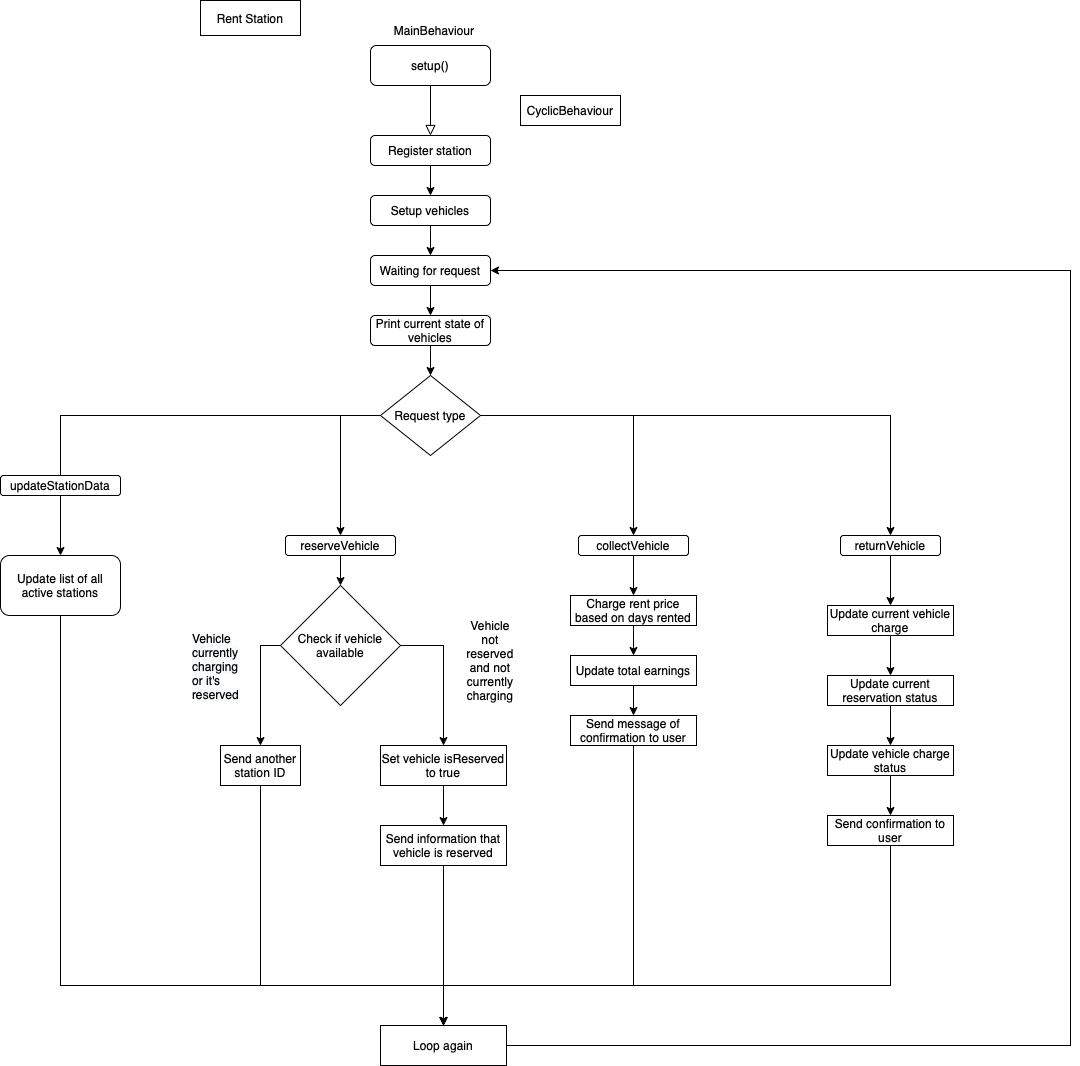
\includegraphics[width=1.0\textwidth]{slike/rentStationSheme.png}
	\caption{Dijagram agenta RentStation (Izvor: U vlastitoj izvedbi, 2022)}
\end{figure}

 \textit{Za potrebe ove simulacije i pojednostavljanje računanja, za parametre u tablicama nisu definirane mjerne jedinice. Sam način računanja prikazan je u implementaciji koda.}

Nakon što se obave podešavanja vozila prelazi se na čekanje zahtjeva. Posljedica zaprimanja novog zahtjeva ispis je trenutnog stanja svih vozila u voznom parku stanice.

\textbf{Update station data} zahtjev stiže od Rent Central agenta nakon što se nova stanica prijavi u sustav najma električnih vozila. Ovim zahtjevom obavještava se stanica sa ažuriranom listom svih aktivnih stanica u sustavu. Nakon zaprimljenog zahtjeva stanica ažurira svoju trenutnu listu.

\textbf{Reserve vehicle zahtjev} pristiže od Rent User agenta koji želi rezervirati određeno vozilo. Stanica provjerava da li je to vozilo dostupno. Dostupnost vozila ovisi o tome je li već prethodno rezervirano i je li trenutno na punjenju ili ne. Ukoliko vozilo nije na punjenju i nije trenutno rezervirano tada se takvo vozilo može unajmiti. U tom slučaju stanica šalje korisniku informaciju o tome da je vozilo uspješno rezervirano. Ukoliko vozilo nije dostupno šalje se sljedeći ID stanice kako bi korisnik mogao poslati zahtjev prema sljedećoj stanici.

\textbf{Collect vehicle zahtjev} pristiže od Rent User agenta koji je došao pokupiti svoje rezervirano vozilo. U ovome trenutku unaprijed se naplaćuje iznos najma električnog vozila ovisno o broju dana koje je korisnik odabrao. Također se ažurira trenutan iznos ukupnih primanja za stanicu. Nakon što su obavljenje ove akcije šalje se potvrda korisniku da je proces gotov, odnosno da korisnik može početi koristiti vozilo.

\textbf{Return vehicle zahtjev} pristiže od Rent User agenta i odnosi se na vraćanje vozila nakon isteka najma. Stanica ažurira trenutnu informaciju vozila o stanju napunjenosti baterije. Nakon toga ažurira se trenutno stanje vozila po pitanju rezervacije i statusu punjenja. Na kraju se šalje potvrda korisniku.

\textbf{Periodično ponašanje} punjenja vozila ponavlja se u jednakim intervalima, te se odnosi na radnje vezane uz punjenje vozila koje su vraćena i koja trenutno nemaju potpuno napunjenu bateriju. Na početku svakog ciklusa ovog ponašanja ispisuje se trenutno stanje vozila i njegovu napunjenost baterijskog sustava. Nakon toga prolazi se kroz listu svih vozila i provjerava se da li je potrebno punjenje bilo kojeg vozila. Ukoliko je potrebno vrši se punjenje u nekom proizvoljnom vremenu. To vrijeme biti će definirano u samoj implementaciji agenata. Nakon što su sva vozila napunjenja takvo će ponašanje biti izvršeno ponovno u zadanom intervalu.

\begin{figure}[h!]
	\centering
	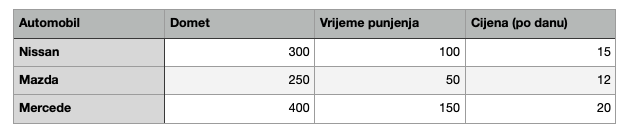
\includegraphics[width=0.7\textwidth]{slike/tablica1.png}
	\caption{Tablica 1: Karakteristike električnih automobila (Izvor: U vlastitoj izvedbi, 2022)}
\end{figure}

\begin{figure}[h!]
	\centering
	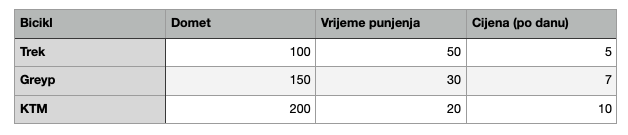
\includegraphics[width=0.7\textwidth]{slike/tablica2.png}
	\caption{Tablica 1: Karakteristike električnih bicikla (Izvor: U vlastitoj izvedbi, 2022)}
\end{figure}

\pagebreak

\section{Rent User Agent}

Agent je definiran kao konačni automat stanja zbog svoje idealne predispozicije. Agent prolazi kroz niz stanja koji su definirani te na posljetku prekida svoj životni vijek. Definirana stanja agenta su:
\begin{itemize}
	\item RESERVE\_VEHICLE
	\item COLLECT\_VEHICLE
	\item USE\_VEHICLE
	\item CHARGE\_VEHICLE
	\item RETURN\_VEHICLE
\end{itemize}

Nakon početne konfiguracije definiraju se tranzicije u kojima se automat može nalaziti. Te su tranzicije navedene u tablici 3.

\begin{figure}[h!]
	\centering
	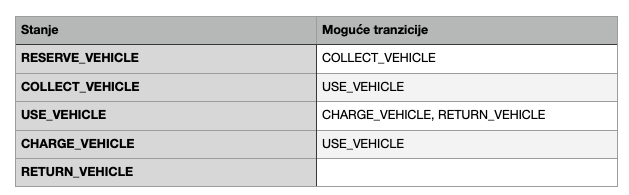
\includegraphics[width=1\textwidth]{slike/tablica3.png}
	\caption{Tablica stanja i prijalaza RentUser agenta (Izvor: U vlastitoj izvedbi, 2022)}
\end{figure}

Sve počinje sa RESERVE\_VEHICLE stanjem u kojem korisnik šalje poruku željenoj stanici da želi rezervirati određeno vozilo na određen broj dana. Ulazni parametri definirani su prilikom pokretanja samog agenta. Nakon toga čeka se na odgovor, a ako je odgovor afirmitivan tada se prelazi u stanje COLLECT\_VEHICLE. Ako odgovor nije afirmitivan mijenja se željena stanica rezervacije i ponovno se prelazi u slanje poruke novoj stanici. 

Nakon što se uspješno rezervira vozilo prelazi se u stanje COLLECT\_VEHICLE gdje korisnik dolazi do određene stanice i preuzima vozilo. U tom trenutku korisnik plaća iznos najamnine vozila. Zatim se prelazi u stanje USE\_VEHICLE gdje korisnik koristi svoje iznajmljeno vozilo sve dok ga ne isprazni. Kada ga isprazni provjerava se da li je moguće i dalje koristiti vozilo, odnosno da li vrijeme koje je ostalo za korištenje vozila je dovoljno da se vozilo napuni i isprazni do kraja. Ukoliko to vrijeme dozvoljava tada prelazimo u stanje CHARGE\_VEHICLE. Ukoliko to vrijeme ne dozvoljava tada se vozilo mora vratiti u stanicu odnosno u stanje RETURN\_VEHICLE. Kod CHARGE\_VEHICLE stanja vozilo se puni do svoje maksimalne razine te se tada ponovno prelazi u stanje USE\_VEHICLE. Kada se prijeđe u stanje RETURN\_VEHICLE tada se javlja stanici da želimo vratiti vozilo, te kada se vozilo vrati završava životni ciklus ovog konačnog automata.

\begin{figure}[h!]
	\centering
	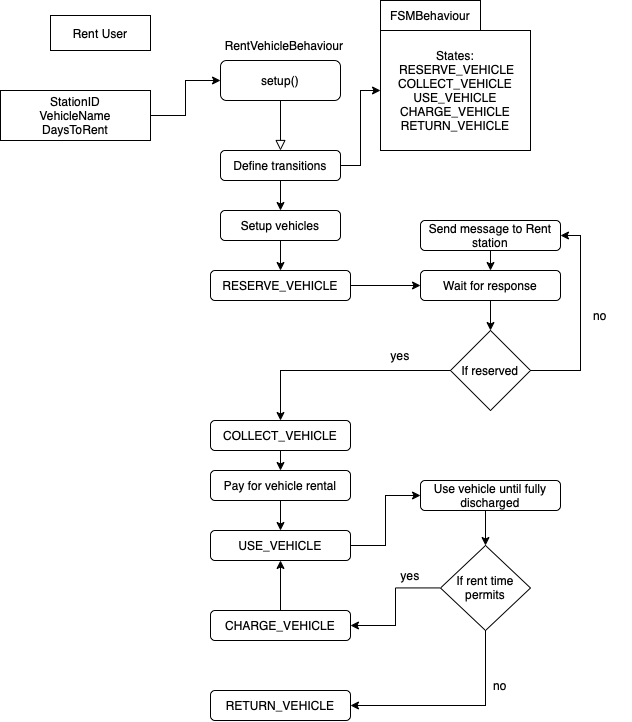
\includegraphics[width=1\textwidth]{slike/rentUser.png}
	\caption{Tablica 1: Dijagram ponašanja RentUser agenta (Izvor: U vlastitoj izvedbi, 2022)}
\end{figure}


\chapter{Implementacija rada}

U ovom dijelu proći će se kroz implementaciju pojedinog agenta u samom kodu. Biti će izdvojeni ključni dijelovi, odnosno ključne zadaće koje izvršavaju pojedini agenti i njihova ponašanja. U prošlom poglavlju detaljno smo prošli kroz dijagrame i izvedbu agenata i njegovih ponašanja te je pojašnjena u detalje njihova uloga i međusobno komunikacija. Izdvojeni su dijelovi koda koja vrše ključne zadaće u agentima.

\section{Rent Central Agent}

Kroz dijagrame ponašanja ovog agenta prošli smo u prošlom poglavlju. Ovdje ćemo proći kroz implementaciju koda za najvažnije dijelove ovog agenta. Ovaj agent ima jedno glavno ponašanje koje je ciklično te služi zaprimanju i obradi zahtjeva od ostalih stanica.

\begin{flushleft}\textbf{MainBehaviour - implementacija čekanja zahtjeva}\end{flushleft}

\begin{lstlisting}[language=Python]
class MainBehaviour(spade.behaviour.CyclicBehaviour):
	async def on_start(self):
	print("I'm starting central behaviour")
	print("--------------")

async def run(self):
	print("Current stations: ", self.agent.stations)
	print("--------------")
	print("Waiting for requests by stations ...")

msg = await self.receive(timeout=100)
	if msg:
		if msg.body == 'registerStation':
			self.agent.stations.append(msg.sender)
			await self.updateStations()
		if msg.body == 'unregisterStation':
			await self.unregisterStation(msg.sender.localpart)
\end{lstlisting}

Ovdje je najveći naglasak na dva zahtjeva koje obrađuje ovaj agent, a to su register i unregisterStation. Nakon zaprimanja zahtjeva registerStation() tada se poziva funkcija updateStations().

\begin{flushleft}\textbf{updateStations()}\end{flushleft}

\begin{lstlisting}[language=Python]
async def updateStations(self):
allStationIDs = []
for station in self.agent.stations:
	allStationIDs.append(station.localpart + "@" + station.domain)

for station in self.agent.stations:
	receiver = station.localpart + "@" + station.domain
	msg = Message(to=receiver)
	msg.set_metadata("performative", "inform")
	msg.set_metadata("ontology", "updateStationData")
	msg.body = ",".join(allStationIDs)
	await self.send(msg)
\end{lstlisting}

U ovom asinkronoj funkciji nakon registracije novo prijavljenje stanice šaljemo informaciju o trenutno svim registiranim stanicama pojedinačno svakoj stanici koja je trenutno aktivna.

\begin{flushleft}\textbf{unregisterStation()}\end{flushleft}

\begin{lstlisting}[language=Python]
async def unregisterStation(self, stationID):
	for station in self.agent.stations:
		if station.localpart == stationID:
			self.agent.stations.remove(station)
	await self.updateStations()
	print("Unregistered station")
\end{lstlisting}

Ova funkcija koristi se kada neka stanica želi izaći iz sustava trenutno aktivnih stanica te se odjavljuje, tj. deregistrira iz sustava. Također poziva se funkcija updateStations() kako bi se trenutni set aktivnih stanica ažurirao kod svake stanice posebno.

\section{Rent Station Agent}

Ovaj agent ima dva ponašanja kroz koja smo prošli u prošlom poglavlju. Glavno ponašanje koje je ciklično te služi zaprimanju i obradi zahtjeva od pojedinačnih klijenata, te također periodično ponašanje koje služi za periodično punjenje baterija električnih vozila.

\begin{flushleft}\textbf{MainBehaviour - on\_start}\end{flushleft}

\begin{lstlisting}[language=Python]
print("I'm starting main behaviour")
print("--------------")
msg = Message(to="lleljak@rec.foi.hr")
msg.set_metadata("performative", "inform")
msg.set_metadata("ontology", "myOntology")
msg.body = "registerStation"
await self.send(msg)
\end{lstlisting}

\begin{flushleft}\textbf{MainBehaviour - on\_end}\end{flushleft}

\begin{lstlisting}[language=Python]
print("Ending agent")
msg = Message(to="lleljak@rec.foi.hr")
msg.set_metadata("performative", "inform")
msg.set_metadata("ontology", "myOntology")
msg.body = "unregisterStation"
await self.send(msg)
\end{lstlisting}

Na početku glavnog ponašanja radimo registraciju stanice u sustav svih aktivnih stanica. Ta poruka šalje se prema Rent Central agentu. Kod završetka ponašanja agenta šalje se unregisterStation poruka koja označava da se ta stanica želi odjaviti iz sustava najma električnih vozila. Takva se poruka također šalje centralnom agentu.

\begin{flushleft}\textbf{MainBehaviour - postavljanje vozila}\end{flushleft}

Tijekom inicijalnog postavljanja agenta, također se postavljaju i vozila. Za potrebe ovog projekta korišten je suženi set vozila svaki sa svojim karakteristikama.

\begin{lstlisting}[language=Python]

class Vehicle:
	def __init__(self, name, maxDistance, chargeTime, pricePerDay):
		self.name = name
		self.maxDistance = maxDistance
		self.charge = 100
		self.chargeTime = chargeTime
		self.pricePerDay = pricePerDay
		self.isReserved = False
		self.isCharging = False

	def printProperties(self): 
		print(self.name, "-", self.charge, "-", self.isReserved)
	
	def printChargeProperties(self): 
		print(self.name, "-", self.charge, "-", self.isCharging)


def setupCars(self):
	return [
		Vehicle("nissan", 300, 100, 15),
		Vehicle("mazda", 250, 50, 12),
		Vehicle("mercedes", 400, 150, 20)
	]

def setupBikes(self):
	return [
		Vehicle("trek", 100, 50, 5),
		Vehicle("greyp", 150, 30, 7),
		Vehicle("ktm", 200, 20, 10)
	]
\end{lstlisting}

\begin{flushleft}\textbf{MainBehaviour - run}\end{flushleft}

Ključna uloga glavnog ponašanja definirano je u run funkciji. Ovo ponašanje zaduženo je za obradu zahtjeva koji pristižu prema RentStation agentu.

\begin{lstlisting}[language=Python]

async def run(self):
	print("------ RENTING SYSTEM BEHAVIOUR ------")
	self.printCurrentState()
	print("Waiting for requests by users ...")
	print("")

	### Handle requests
	msg = await self.receive(timeout=100)
	if msg and msg.metadata:
		if msg.metadata["ontology"] == 'updateStationData':
			self.agent.stations = msg.body.split(",")
		if msg.metadata["ontology"] == 'reserveVehicle':
			vehicleName = msg.body
			await self.reserveVehicle(vehicleName, msg.sender)
		if msg.metadata["ontology"] == 'collectVehicle':
			vehicleName = msg.body.split(",")[0]
			days = msg.body.split(",")[1]
			await self.collectVehicle(vehicleName, int(days), msg.sender)
		if msg.metadata["ontology"] == 'returnVehicle':
			vehicleName = msg.body.split(",")[0]
			chargeLeft = msg.body.split(",")[1]
			await self.returnVehicle(vehicleName, chargeLeft, msg.sender)

\end{lstlisting}

\begin{flushleft}\textbf{MainBehaviour - reserveVehicle}\end{flushleft}

Funkcijom reserveVehicle obrađuje se zahtjev klijenta za rezerviranjem vozila. Pronalazi se vozilo koje korisnik želi rezervirati i ukoliko je rezervacija moguća (prema pravilima definiranim u prethodnom poglavlju) vrši se rezervacija vozila. Ukoliko se vozilo ne može rezervirati tada se šalje id neke druge stanice korisniku kako bi mogao poslati zahtjev na drugu adresu. Ukoliko se vozilo može rezervirati, šalje se potvrdna poruka o rezervaciji željenog vozila.

\begin{lstlisting}[language=Python]

### Reserve vehicle for customer
###
async def reserveVehicle(self, vehicleName, sender):
	for vehicle in self.agent.vehicles:
		if vehicle.name == vehicleName:
			if not vehicle.isReserved and not vehicle.isCharging:
				vehicle.isReserved = True
				canReserveVehicle = True
			else:
				canReserveVehicle = False
			break
	reservationStation = str(self.agent.jid)

if canReserveVehicle:
	msg = Message(to=sender.localpart + "@" + sender.domain)
	msg.set_metadata("performative", "inform")
	msg.set_metadata("ontology", "vehicleReserved")
	msg.body = reservationStation
	await self.send(msg)
else:
	numberOfStations = len(self.agent.stations) - 1
	if numberOfStations == 0:
		msg = Message(to=sender.localpart + "@" + sender.domain)
		msg.set_metadata("performative", "inform")
		msg.set_metadata("ontology", "noOtherStations")
		msg.body = reservationStation
		await self.send(msg) 
	else:
		randomStation = random.randint(0, numberOfStations)
		reservationStation = self.agent.stations[randomStation].partition("@")[0]
		msg = Message(to=sender.localpart + "@" + sender.domain)
		msg.set_metadata("performative", "inform")
		msg.set_metadata("ontology", "otherStation")
		msg.body = reservationStation
		await self.send(msg) 
		print("Vehicle can't be reserved, sending another station details to customer...")

\end{lstlisting}

\begin{flushleft}\textbf{MainBehaviour - collectVehicle}\end{flushleft}

Funkcijom collectVehicle korisnik javlja da je došao preuzeti vozilo. U tom trenutku također korisnik i plaća vozilo, te se ažurira ukupna zarada stanice. Također šalje se potvrdna poruka prema klijentu.

\begin{lstlisting}[language=Python]

### Customer collects vehicle
###
async def collectVehicle(self, vehicleName, days, sender):
	for vehicle in self.agent.vehicles:
		if vehicle.name == vehicleName:
			self.agent.totalEarnings += days * vehicle.pricePerDay
			break
	
	msg = Message(to=sender.localpart + "@" + sender.domain)
	msg.set_metadata("performative", "inform")
	msg.set_metadata("ontology", "vehicleCollected")
	msg.body = str(self.agent.totalEarnings)
	await self.send(msg)

\end{lstlisting}

\begin{flushleft}\textbf{MainBehaviour - returnVehicle}\end{flushleft}

Funkcijom returnVehicle korisnik javlja da je došao vratiti vozilo. Vozilo se stavlja u red na čekanje punjenja, te se njegova zastavica stanja rezervacije postavlja na false. Također se šalje potvrdna poruka prema klijentu.

\begin{lstlisting}[language=Python]

 ### Customer returns vehicle
###
async def returnVehicle(self, vehicleName, chargeLeft, sender):
	for vehicle in self.agent.vehicles:
	if vehicle.name == vehicleName:
			vehicle.charge = int(float(chargeLeft))
			vehicle.isCharging = True
			vehicle.isReserved = False
			break
	
	msg = Message(to=sender.localpart + "@" + sender.domain)
	msg.set_metadata("performative", "inform")
	msg.set_metadata("ontology", "vehicleReturned")
	msg.body = vehicleName
	await self.send(msg)

\end{lstlisting}

\begin{flushleft}\textbf{ChargingBehaviour}\end{flushleft}

Funkcijom returnVehicle korisnik javlja da je došao vratiti vozilo. Vozilo se stavlja u red na čekanje punjenja, te se njegova zastavica stanja rezervacije postavlja na false. Također se šalje potvrdna poruka prema klijentu.

\begin{lstlisting}[language=Python]

async def on_start(self):
	print("I'm starting charging behaviour")

async def run(self):
	print("------ CHARGING BEHAVIOUR ------")
	self.printCurrentState()

	needsCharging = False
### Charge vehicles if needed
	for vehicle in self.agent.vehicles:
		if vehicle.charge < 100:
			needsCharging = True
			break
	
	if needsCharging:
		print("Started charging vehicles")
		await asyncio.sleep(20)
		for vehicle in self.agent.vehicles:
		vehicle.charge = 100
		vehicle.isCharging = False
		print("All vehicles charged")
	else:
		print("No need to charge vehicles")
	
	print("")

\end{lstlisting}

Periodično ponašanje punjenja vozila ponavlja se u jednakim intervalima, te se odnosi na radnje vezane uz punjenje vozila koje su vraćena i koja trenutno nemaju potpuno napunjenu bateriju. Na početku svakog ciklusa ovog ponašanja ispisuje se trenutno stanje vozila i njegovu napunjenost baterijskog sustava. Nakon toga prolazi se kroz listu svih vozila i provjerava se da li je potrebno punjenje bilo kojeg vozila. Ukoliko je potrebno vrši se punjenje u nekom proizvoljnom vremenu. Nakon što su sva vozila napunjenja takvo će ponašanje biti izvršeno ponovno u zadanom intervalu.

\section{Rent User Agent}

Ovaj agent kreiran je kao konačni automat stanja zbog svoje savršene predispozicije. Prijelaz iz stanja u stanje, te moguće tranzicije definirane su u prethodnom poglavlju gdje je detaljnije opisana arhitektura sustava. Ovdje ćemo proći kroz implementaciju konkretnih stanja u kodu.

\begin{flushleft}\textbf{RESERVE\_VEHICLE stanje}\end{flushleft}

Sa ovim stanjem počinje agent. Iz ovog stanje može ponovno prijeći u svoje stanje ili prelazi u stanje COLLECT\_VEHICLE.

\begin{lstlisting}[language=Python]
 ## Tell station that you want to reserve it - if it's unavailable station will give you
## other station from list.
##
print("------ RESERVE VEHICLE ------ ")
print("Going to collect vehicle at station -", self.agent.station, STATION_ADDRESS)
msg = Message(to=self.agent.station + STATION_ADDRESS)
msg.set_metadata("performative", "inform")
msg.set_metadata("ontology", "reserveVehicle")
msg.body = self.agent.vehicle
await self.send(msg)
print("Waiting for response...")
msgReceived = await self.receive(timeout=10000)
self.agent.station = msgReceived.body

if msgReceived and msgReceived.metadata:
	if msgReceived.metadata["ontology"] == 'vehicleReserved':
		print("Vehicle ", self.agent.vehicle, " is reserved at station ", msgReceived.body)
		print("Going to station ...")
		time.sleep(2)
		self.set_next_state(COLLECT_VEHICLE)
	elif msgReceived.metadata["ontology"] == 'noOtherStations':
		print("No other stations available, finishing agent...")
		time.sleep(2)
		self.kill()
	elif msgReceived.metadata["ontology"] == 'otherStation':
		self.agent.station = msgReceived.body
		self.set_next_state(RESERVE_VEHICLE)
\end{lstlisting}

Prijelaz stanja ovisi o tome da li je korisnik uspješno rezervirao vozilo kod željene stanice. Ako je dobio povratnu informaciju sa novim id-em stanice tada ponovno prelazi u isto stanje i ponovno šalje zahtjev za rezervacijom na novu adresu stanice. Ukoliko dobiva povratnu informaciju da nema drugih stanica u blizini agent završava sa svojim radom.

\begin{flushleft}\textbf{COLLECT\_VEHICLE stanje}\end{flushleft}

Ukoliko je agent uspješno rezervirao vozilo, prelazi u stanje COLLECT\_VEHICLE, te iz tog stanja prelazi u USE\_VEHICLE stanje ukoliko je dobiven afirmativan odgovor.

\begin{lstlisting}[language=Python]
## Tell station that you collected vehicle and pay at advance
##
print("\n------ COLLECT VEHICLE ------ ")
print("Arrived at station")
msg = Message(to=self.agent.station)
msg.set_metadata("performative", "inform")
msg.set_metadata("ontology", "collectVehicle")
msg.body = ",".join([self.agent.vehicle, self.agent.days])
await self.send(msg)

print("Waiting for response...")
msgReceived = await self.receive(timeout=10000)
print("Vehicle is collected and rent is payed", msgReceived.body, "€")
\end{lstlisting}

\begin{flushleft}\textbf{USE\_VEHICLE stanje}\end{flushleft}

U ovom stanju agent koristi vozilo sve dok se njegova baterija ne isprazni. Korištena je skraćena logika vremena u sekunda podijeljena sa 10 tako da se ne treba dugo čekati kada se simulacija pokreće. 

\begin{lstlisting}[language=Python]
## Random usage, random charging after it's used and etc
## From this state to Charge or to ReturnVehicle
##
print("\n------ USE VEHICLE ------ ")
print("I'm using vehicle")

for vehicleF in self.agent.vehicles:
	if vehicleF.name == self.agent.vehicle:
		vehicleChargeTime = vehicleF.chargeTime / 10
		vehicleRange = vehicleF.maxDistance
		break

fullRangeTime = vehicleRange/10
time.sleep(fullRangeTime)
print("Vehicle fully discharged")
self.agent.daysRemaining -= fullRangeTime
print("Rent time remaining:", self.agent.daysRemaining)

if self.agent.daysRemaining >= fullRangeTime + vehicleChargeTime:
	self.set_next_state(CHARGE_VEHICLE)    
else:
	self.set_next_state(RETURN_VEHICLE)    
\end{lstlisting}

Kada korisnik vozilo isprazni provjerava se da li je moguće i dalje koristiti vozilo, odnosno da li vrijeme koje je ostalo za korištenje vozila je dovoljno da se vozilo napuni i isprazni do kraja. Ukoliko to vrijeme dozvoljava tada prelazimo u stanje CHARGE\_VEHICLE. Ukoliko to vrijeme ne dozvoljava tada se vozilo mora vratiti u stanicu odnosno u stanje RETURN\_VEHICLE.

\begin{flushleft}\textbf{CHARGE\_VEHICLE stanje}\end{flushleft}

\begin{lstlisting}[language=Python]
 ## Charging the vehicle
##
print("\n------ CHARGE VEHICLE ------ ")
print("I'm charging vehicle")
for vehicle in self.agent.vehicles:
	if vehicle.name ==  self.agent.vehicle:
		vehicleChargeTime = vehicle.chargeTime / 10
time.sleep(vehicleChargeTime)
self.agent.daysRemaining -= vehicleChargeTime
print("Vehicle charged to 100%")
print("Rent time remaining:", self.agent.daysRemaining)
self.set_next_state(USE_VEHICLE)
\end{lstlisting}

U ovom stanju korisnik stavlja vozilo na punjenje. Nakon toga prolazi se u USE\_VEHICLE stanje.

\begin{flushleft}\textbf{RETURN\_VEHICLE stanje}\end{flushleft}

Kada je vrijeme najma vozila isteklo tada se prelazi u ovo stanje gdje se šalje zahtjev prema stanici gdje je vozilo iznajmljeno da se vozilo vraća. Također se u takvoj poruci šalje i informacija o tome koliko je trenutno baterije ostalo u vozilu kako bi stanica imala takav podatak i mogla ažurirati svoje stanje.

\begin{lstlisting}[language=Python]
 ## Tell station that you are giving it back and how much charge is left
##
print("\n------ RETURN VEHICLE ------ ")
print("I'm returning vehicle")
msg = Message(to=self.agent.station)
msg.set_metadata("performative", "inform")
msg.set_metadata("ontology", "returnVehicle")
msg.body = ",".join([self.agent.vehicle, str(self.agent.daysRemaining)])
print("Returning vehicle", self.agent.vehicle, "with charge left:", self.agent.daysRemaining)
await self.send(msg)

print("Waiting for response...")
msgReceived = await self.receive(timeout=10000)
print("Vehicle returned succesfully, heading home...")
time.sleep(2)
\end{lstlisting}

\chapter{Prikaz rada aplikacije}

U ovom poglavlju proći ćemo kroz neke primjere korištenja aplikacije. Za početak ćemo pokrenuti glavni centralni agenta, a to je RentCentral.

\begin{figure}[H]
    \centering
    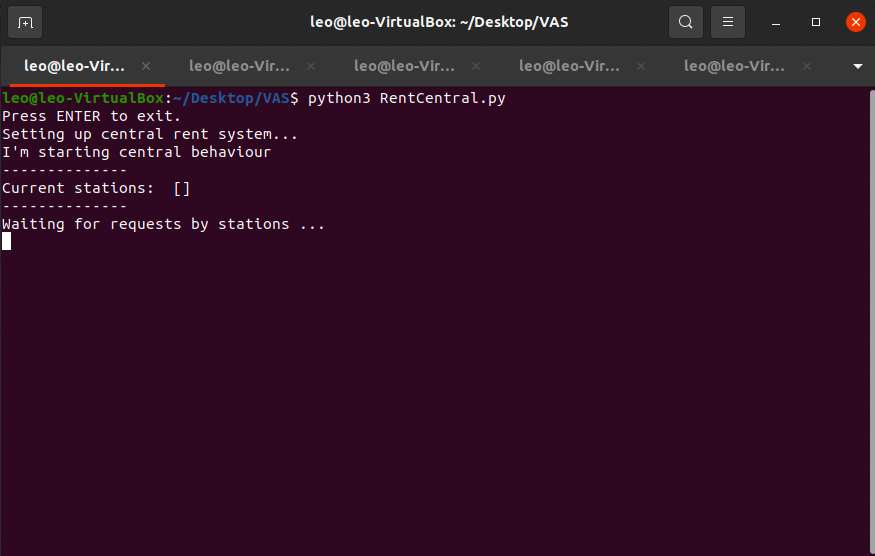
\includegraphics[width=0.8\textwidth]{slike/vas1}
    \caption{RentCentral pokretanje (Izvor: u vlastitoj izvedbi (snimka zaslona), 2022)}
\end{figure}

Nakon što se pokrene centralni program on ispisuje trenutno prijavljene stanice koje su trenutno dostupne. Trenutno nema prijavljenih stanica pa je takva lista prazna. Potrebno je pokrenuti sljedećeg agenta, a to je RentStation. U ovom ćemo primjeru pokrenuti ukupno dvije različite stanice.

\begin{figure}[H]
	\centering
	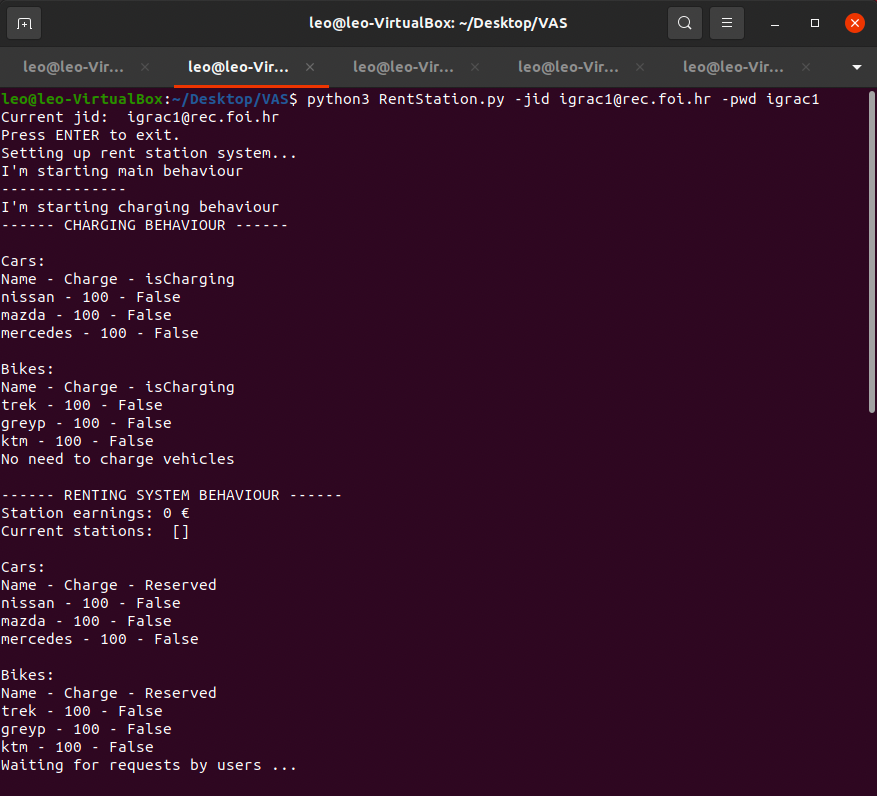
\includegraphics[width=0.8\textwidth]{slike/vas2}
	\caption{Pokretanje stanice A (Izvor: u vlastitoj izvedbi (snimka zaslona), 2022)}
\end{figure}

\begin{figure}[H]
	\centering
	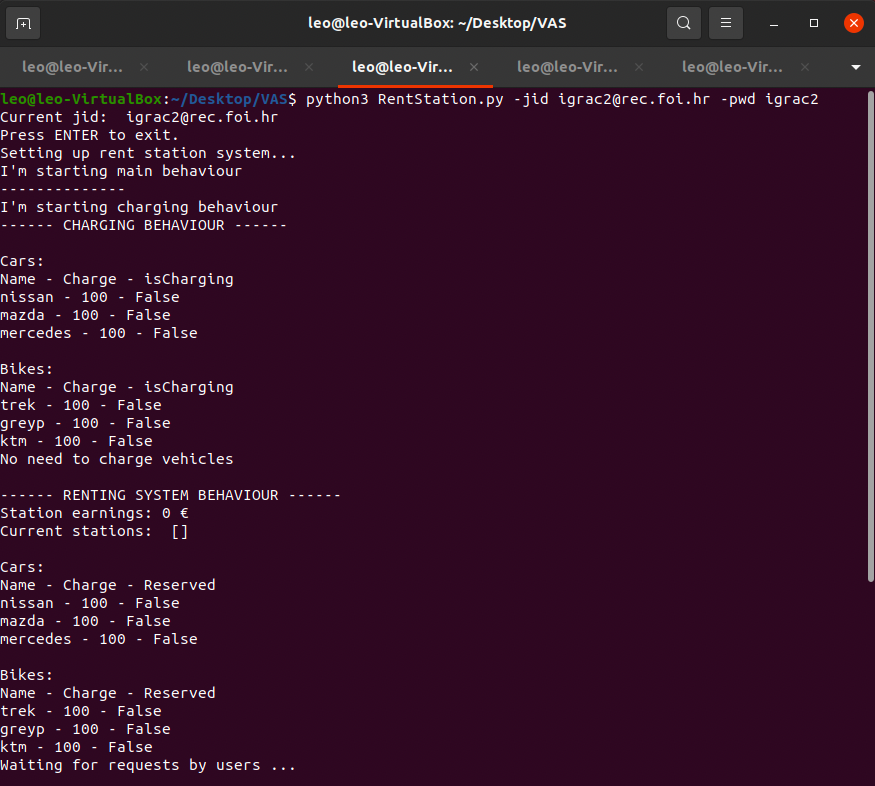
\includegraphics[width=0.8\textwidth]{slike/vas3}
	\caption{Pokretanje stanice B (Izvor: u vlastitoj izvedbi (snimka zaslona), 2022)}
\end{figure}

Nakon što se takve stanice pokrenu pokreću se i njihova ponašanja, te se ispisuje trenutno stanje vozila kao i stanje na punjenju. U ovome trenutku imamo pokrenuto ukupno tri agenata od koji je jedan centralni, dok su dva stanice koje pružaju usluge. 

Ukoliko sada pogledamo centralnog agenta možemo vidjeti da je on registrirao obje stanice te da ima podatke o njima. 

\begin{figure}[H]
	\centering
	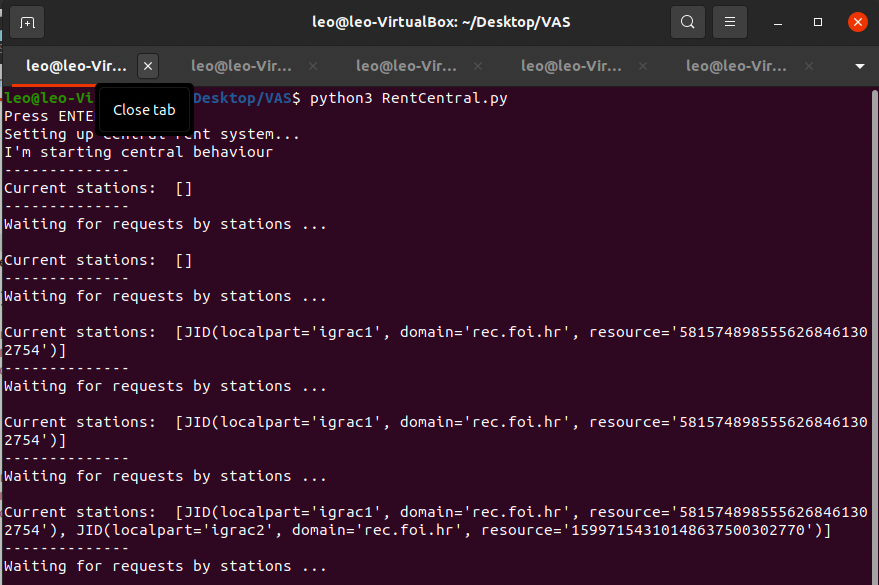
\includegraphics[width=0.8\textwidth]{slike/vas4}
	\caption{RentCentral pregled trenutnih stanica (Izvor: u vlastitoj izvedbi (snimka zaslona), 2022)}
\end{figure}

Također kod prve stanice, zovimo je \textbf{stanica A} možemo vidjeti da ona ima također znanja o svim trenutno registiranim stanicama.

\begin{figure}[H]
	\centering
	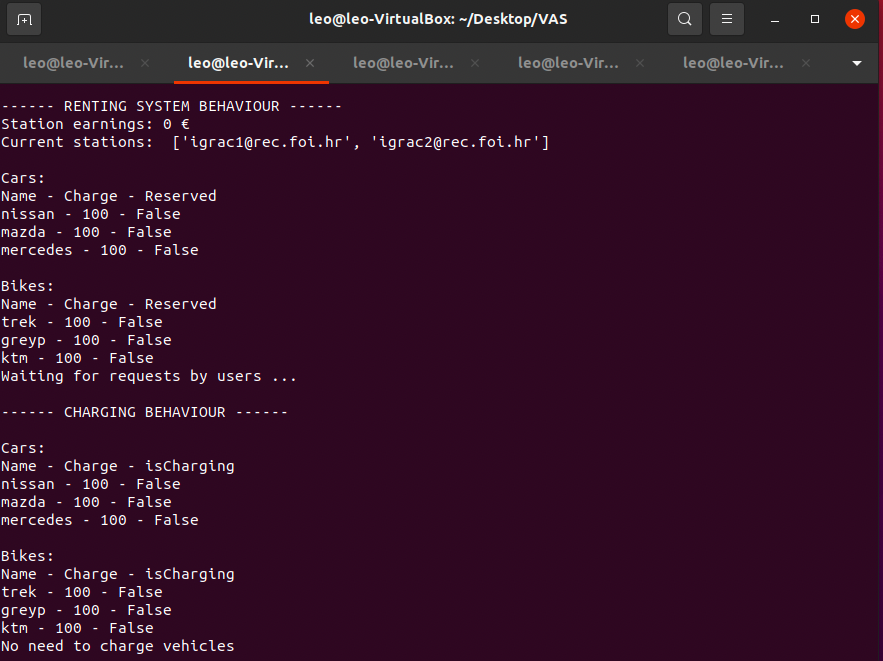
\includegraphics[width=0.8\textwidth]{slike/vas5}
	\caption{Stanica A - prikaz svih stanica (Izvor: u vlastitoj izvedbi (snimka zaslona), 2022)}
\end{figure}

Kod \textbf{stanice B} imamo isti slučaj, ona također je zaprimila poruku od glavne stanice te ima podatke o trenutno svim prijavljenim stanicama u sustav.

\begin{figure}[H]
	\centering
	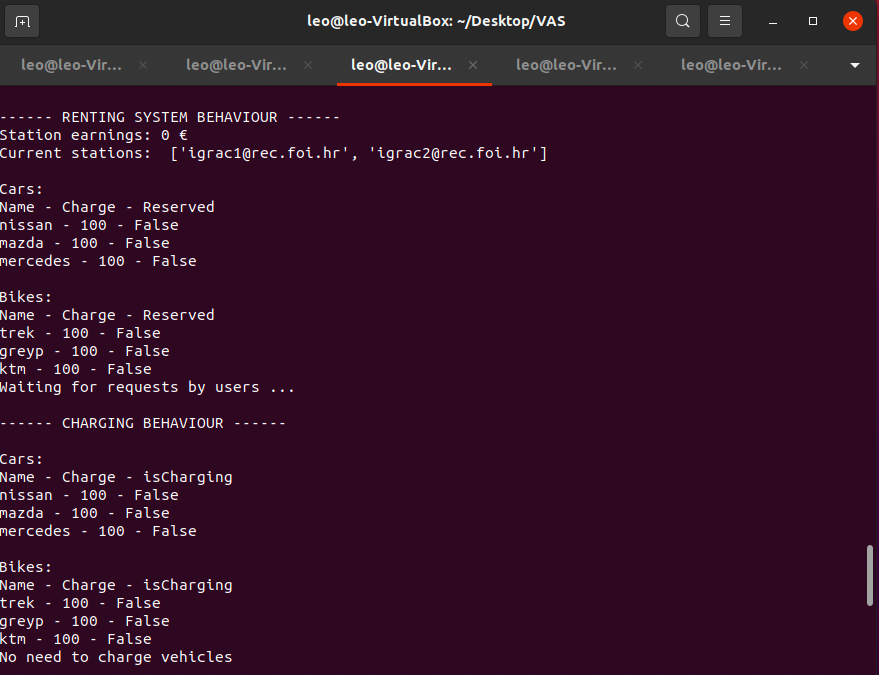
\includegraphics[width=0.8\textwidth]{slike/vas6}
	\caption{Stanica B - prikaz svih stanica(Izvor: u vlastitoj izvedbi (snimka zaslona), 2022)}
\end{figure}

Sad kad imamo spremno sve kako bismo mogli iznajmiti električno vozilo, pokrenimo zahtjev za najmom električnog vozila preko agenta RentUser. Pokrenuti ćemo zahtjev za vozilom mazda i želimo ga rezervirati na 1 dan.

python3 RentUser.py -jid agent@rec.foi.hr -pwd tajna -station igrac1 -vehicle mazda -days 1

Zahtjev se šalje stanici A.

\pagebreak

\begin{figure}[H]
	\centering
	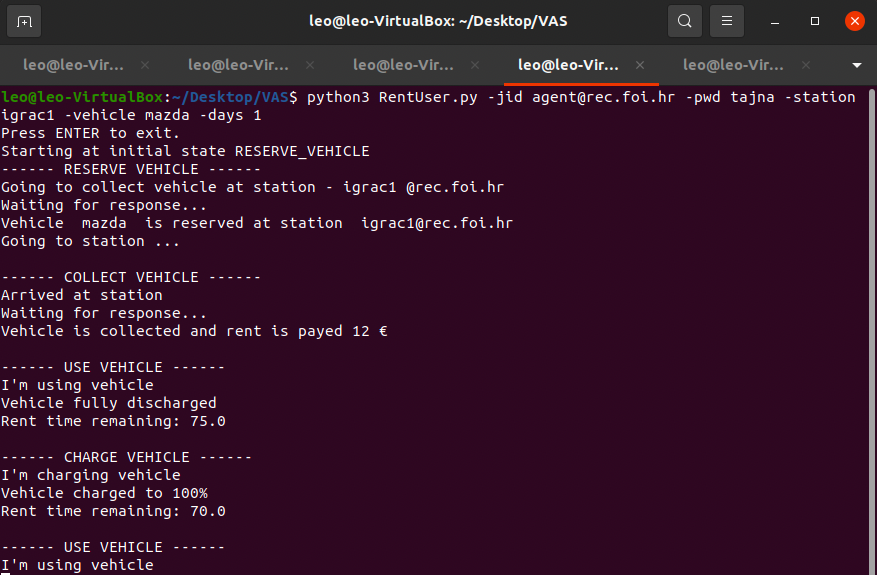
\includegraphics[width=0.8\textwidth]{slike/vas7}
	\caption{UserRent zahtjev za najmom vozila(Izvor: u vlastitoj izvedbi (snimka zaslona), 2022)}
\end{figure}

\begin{figure}[H]
	\centering
	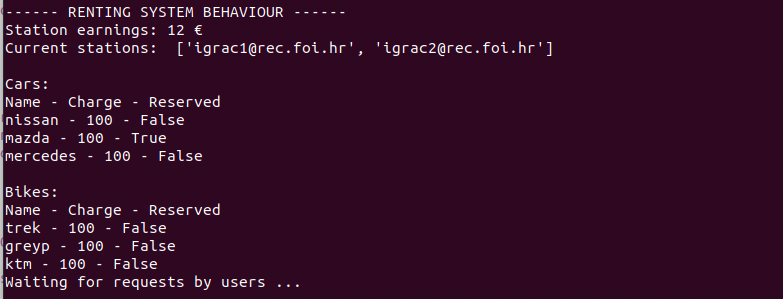
\includegraphics[width=0.8\textwidth]{slike/vas8}
	\caption{Stanica A pruža najam vozila korisniku (Izvor: u vlastitoj izvedbi (snimka zaslona), 2022)}
\end{figure}

Na gornje dvije slike može se vidjeti kako je zahtjev obrađen te je korisnik uspješno rezervirao vozilo kod stanice A. Stanica A promijenila je stanje vozila u rezervirano, te je nakon toga korisnik došao pokupiti svoje vozilo. Nakon toga stanica je uspješno naplatila najam vozila te se je trenutno stanje ukupne zarade promijenilo sukladno troškovima. Korisnik je počeo koristiti vozilo te se na slici vidi jedna iteracija korištenja gdje je korisnik ispraznio vozilo do kraja, napunio ga i ponovno počeo koristiti vozilo. Sada ćemo pogledati kako izgleda kraj korištenja kada više korisnik nema vremena za korištenje vozila, odnosno vrijeme najma je isteklo.

\begin{figure}[H]
	\centering
	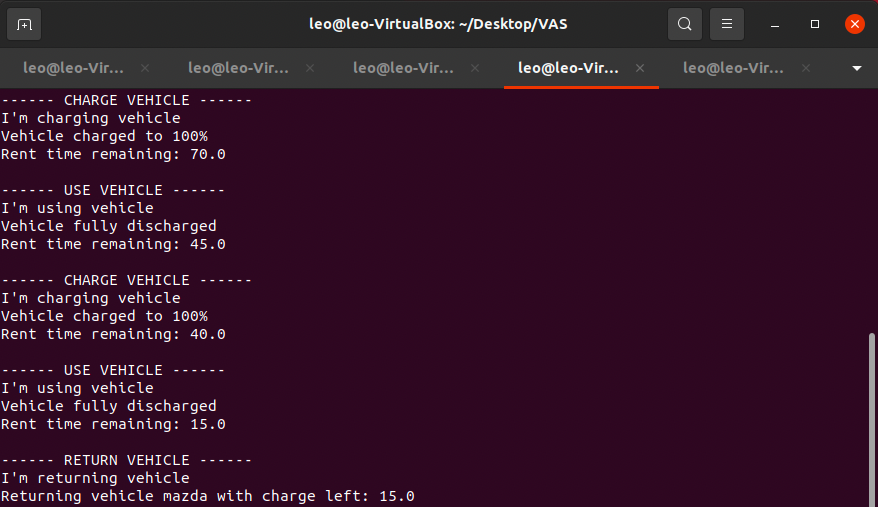
\includegraphics[width=0.8\textwidth]{slike/vas9}
	\caption{Vraćanje vozila (Izvor: u vlastitoj izvedbi (snimka zaslona), 2022)}
\end{figure}

Kada je vrijeme isteklo korisnik je vratio vozilo u stanicu.

\pagebreak

\begin{figure}[H]
	\centering
	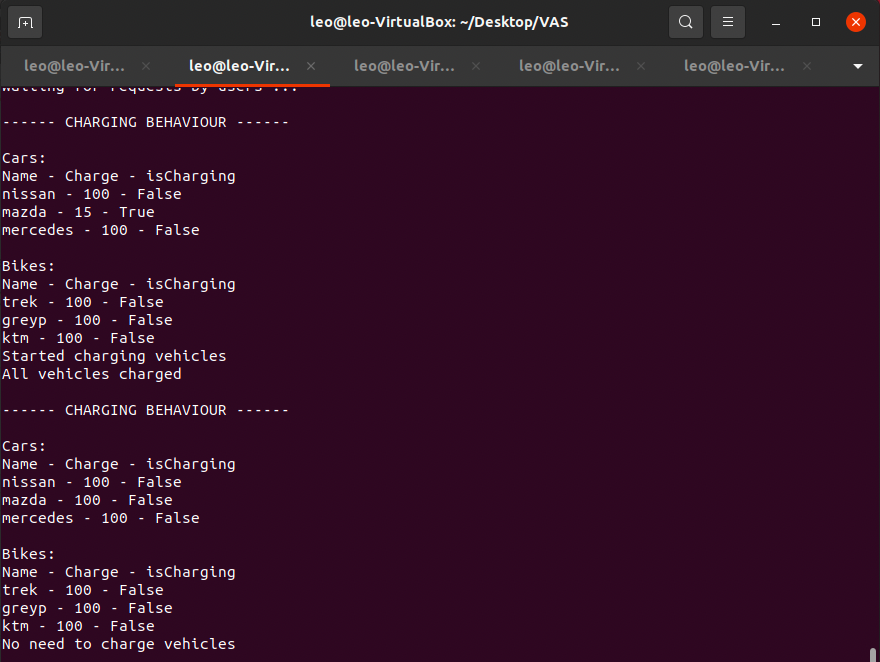
\includegraphics[width=0.8\textwidth]{slike/vas10}
	\caption{Ponašanje punjenja kod Stanice A (Izvor: u vlastitoj izvedbi (snimka zaslona), 2022)}
\end{figure}

Stanica je obradila zahtjev te se vozilo stavilo na punjenje. Na gornjoj slici možemo vidjeti da je pokrenuto ponašanje punjenja, te su sada sva vozila kojima je bilo potrebno punjenje napunjena.

Također proći ćemo kroz još jedan primjer u radu aplikacije. Naime ukoliko korisnik iznajmi vozilo, te drugi korisnik želi iznajmiti isto to vozilo na istoj stanici takvo vozilo nije dostupno. U tom će ga slučaju stanica A preusmjeriti u stanicu B te će korisnik uspješno rezervirati vozilo u drugoj stanici što možemo vidjeti na potonjoj slici.

\begin{figure}[H]
	\centering
	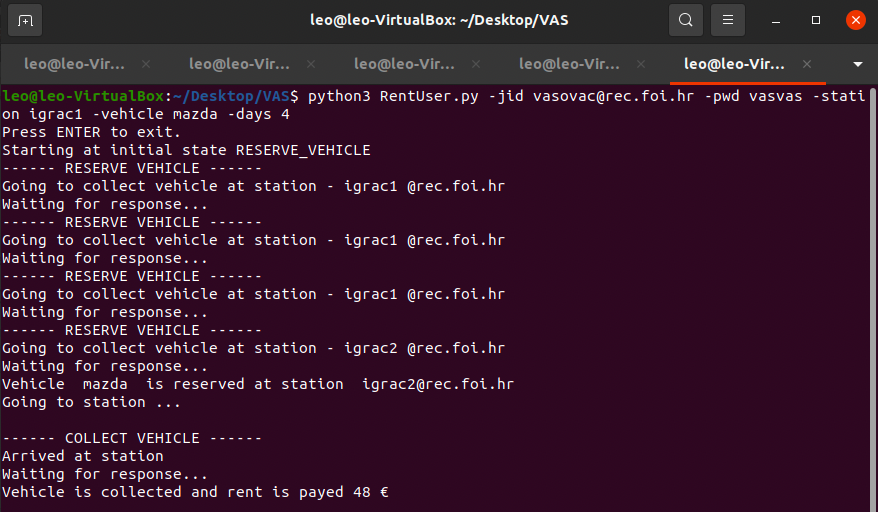
\includegraphics[width=0.8\textwidth]{slike/vas11}
	\caption{Prikaz rezervacije prema usmjerenoj stanici B (Izvor: u vlastitoj izvedbi (snimka zaslona), 2022)}
\end{figure}


\chapter{Zaključak}

Prikazanim sustavom najma električnih vozila ostvaren je cilj projektnog zadatka gdje je glavni fokus na međusobnu komunikaciju agenata i njihovu suradnju. Gotovo svaki agent imao je mogućnost zaprimanja zahtjeva, ali je i slao zahtjeve prema drugim agentima. Pokušaj decentralizacije sustava je uspio na način da svaka stanica je neovisna, te može raditi i ukoliko glavni centar prestane sa svojim radom. Sustav je pojednostavljen kako bi se veća pozornost svela na međusobnu komunikaciju agenata i na implementaciju raznih ponašanja kod istih. U ovome radu korištene su različite vrste ponašanja poput cikličnog, periodičnog, te konačni automat stanja. Konačni automat stanja bio mi je najzanimljivi od njih zbog svoje specifičnosti izvedbe gdje su stanja unaprijed jasno definirana i moguće je lako prenijeti zamišljeno u kod. Ciklično ponašanje uglavnom se koristilo kod zaprimanja i obrade zahtjeva zbog potrebe da se takva radnja vrti u krug i da agenti mogu ponovno zaprimiti novi zahtjev. 

\chapter{Popis literature}

[1] SPADE documentation. Preuzeto sa https://spade-mas.readthedocs.io/en/latest/readme.html.

[2] M. Beer, M. Inverno, M. Luck, N. Jennings, C. Preist i M. Schroeder, Negotiation in Multi- Agent Systems, 1999.

[3] Multi-Agent Vehicle Share System, Roman i ostali, 2019, Preuzeto sa https://www.researchgate.net/publication/338146474\_Multi-Agent\_Vehicle\_Share\_System

\printbibliography[title=Popis literature]
\addcontentsline{toc}{chapter}{Popis literature}

\listoffigures
\addcontentsline{toc}{chapter}{Popis slika}

\appendix
\renewcommand{\thechapter}{\arabic{chapter}}

\chapter{Prilozi}

\begin{itemize}
    \item RentCentral.py
    
    \item RentStation.py
    
    \item RentUser.py
\end{itemize}


\end{document}
